\appendix

\renewcommand{\headrulewidth}{1pt}
\chapter{Annexe}



\section{Diagramme d'interaction << Modifier \'ev\'enement >>}

Dans la Figure \ref{modifierevent}, nous pr\'esentons le diagramme d'interaction du cas d'utilisation << Modifier \'ev\'enement >>. 

Depuis la vue globale, l'utilisateur choisit quel \'ev\'enement veut-il modifi\'e. Par la suite, il est redirig\'e vers l'interface "Modifier \'ev\'enement" pour saisir les nouvelles informations. En validant ses choix, une v\'erification de la saisie est effectu\'ee. Si l'utilisateur se trompe, il sera invit\'e \`a ressaisir les donn\'ees introduites. Au cas contraire, le syst\`eme envoie les nouvelles informations \`a la classe <<contr\^ole \'ev\'enement>> qui se chargera de modifier l'\'ev\'enement concern\'e. Une notification est affich\'ee \`a l'utilisateur que la modification a \'et\'e effectu\'ee avec succ\'es. Suite \`a \c{c}a, la vue "Modifier \'ev\'enement" sera d\'etruite. L'utilisateur sera redirig\'e vers la "Vue Globale" qui sera, par cons\'equant, actualis\'ee.  
\begin{landscape}
\begin{figure}[H]
	\centering
		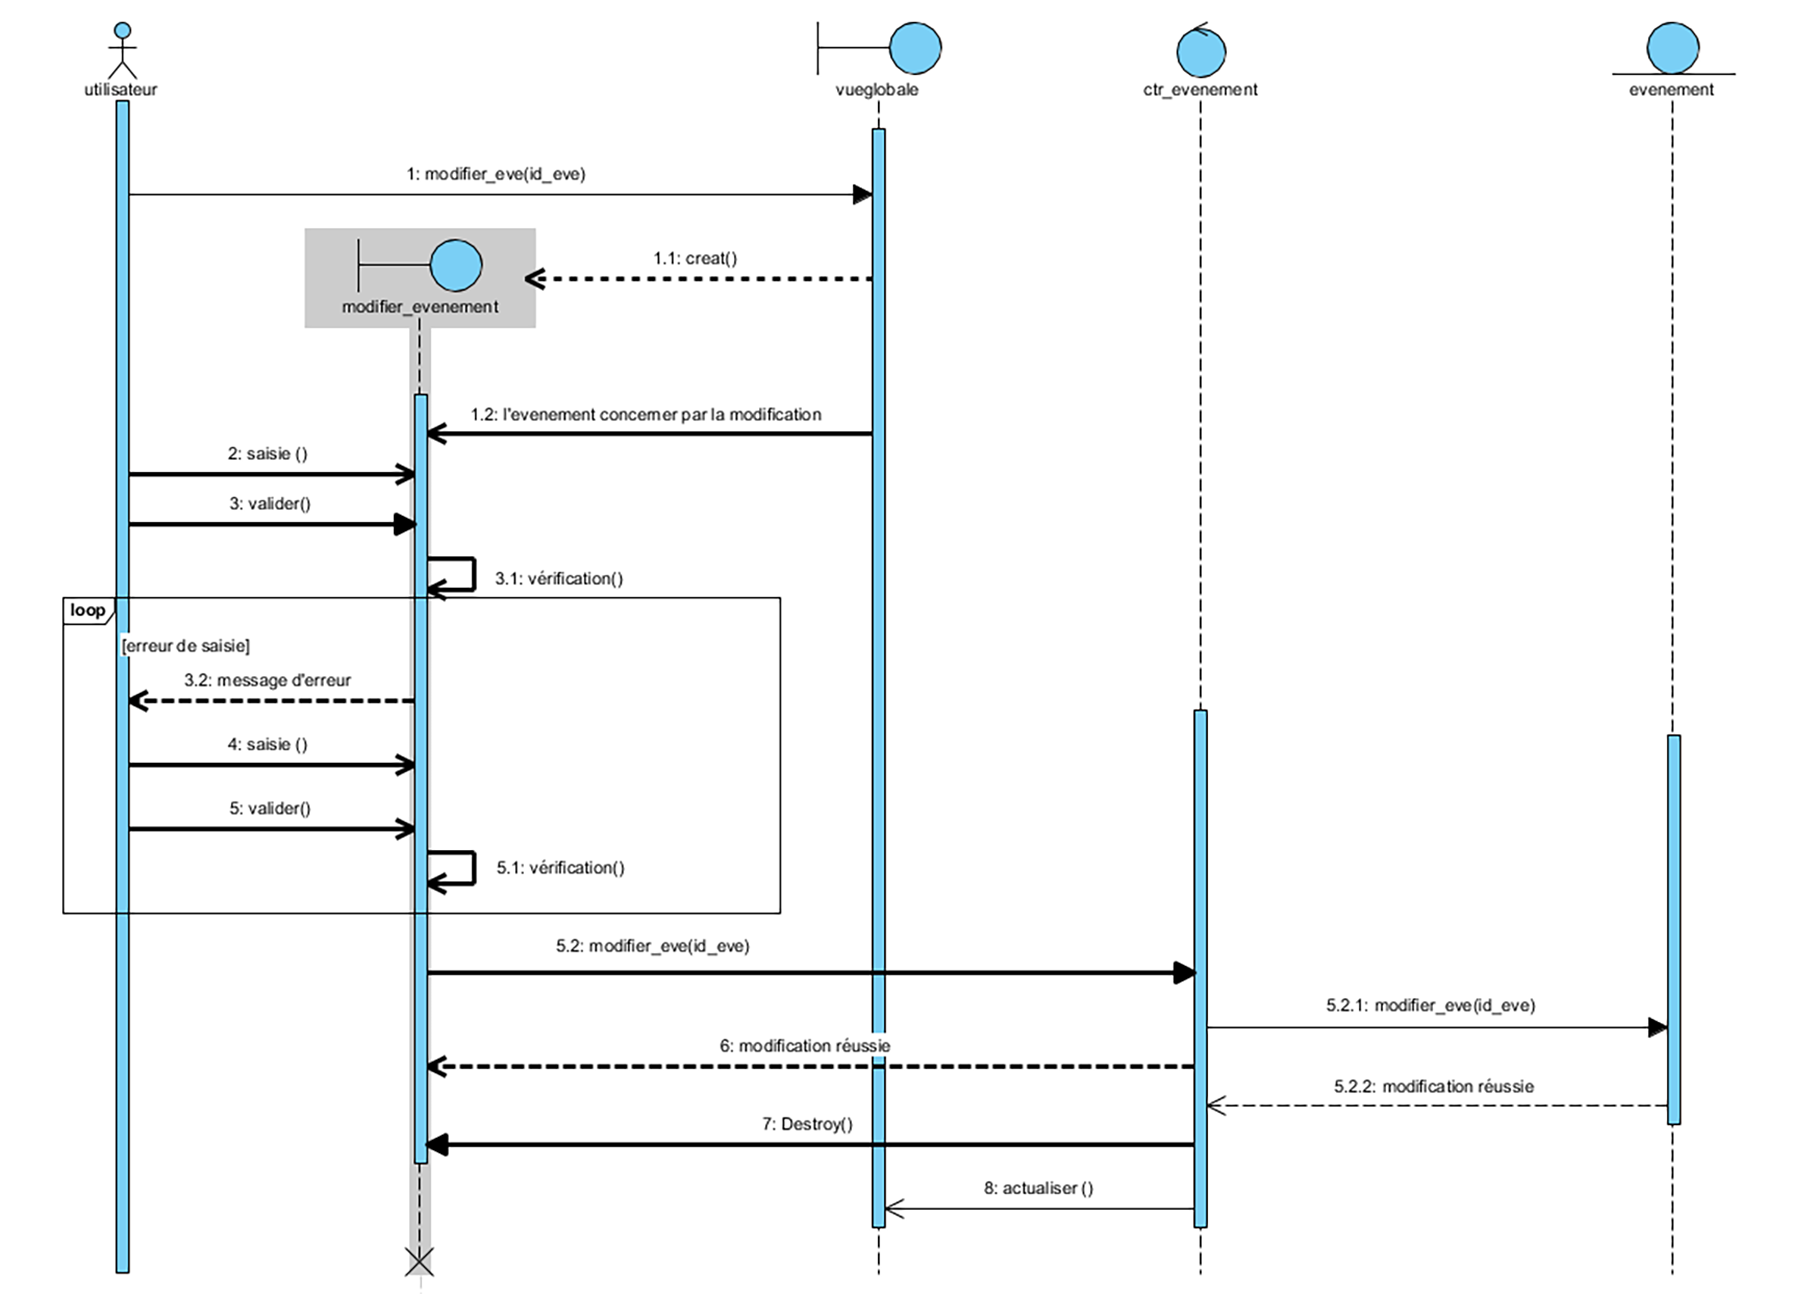
\includegraphics[width=21cm]{images/modifier_event.PNG}
	\caption{Diagramme d'interaction << Modifier \'ev\'enement >>.}
	\label{modifierevent}
\end{figure}
\end{landscape}

\section{Interfaces de l'application}

La Figure \ref{menulateral} repr\'esente le menu lat\'eral qui permet de naviguer entre les diff\'erentes activit\'es de l'application.

La Figure \ref{menuoption} repr\'esente le menu d'option, il permet \`a l'utilisateur de choisir le nombre de jours \`a afficher dans la vue globale.
\begin{figure}[H]
\centering
	
	\subfigure[Menu lat\'eral]{\label{menulateral}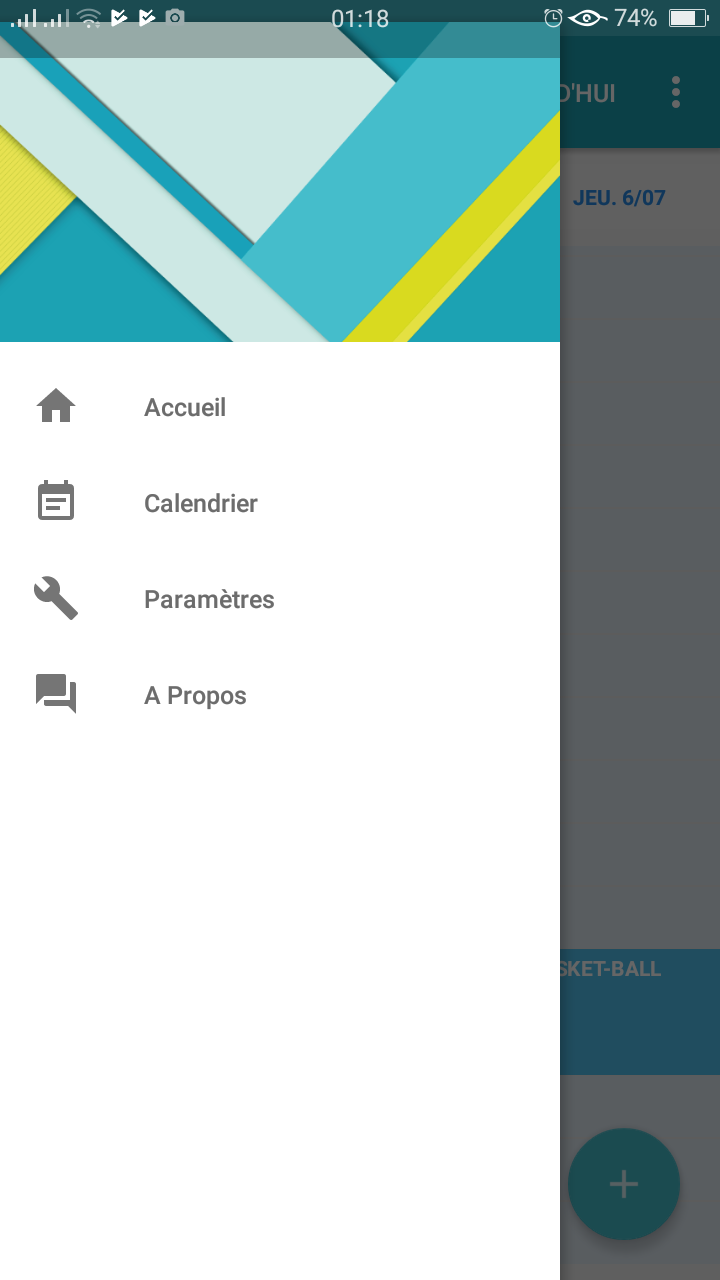
\includegraphics[width=5cm]{images/menu_lateral.png}}
	\subfigure[Menu Option]{\label{menuoption}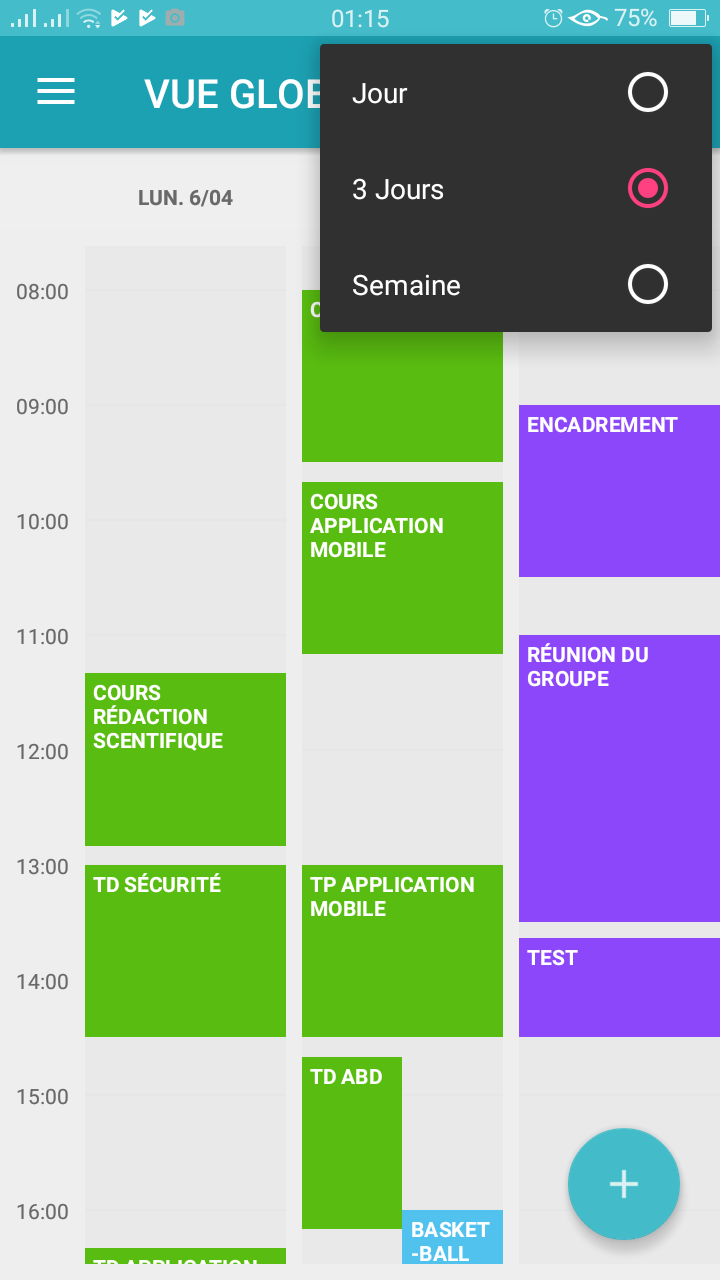
\includegraphics[width=5cm]{images/menu_droite.png}}
		
	\caption{Les menus lat\'eraux}
	\label{home}
	
\end{figure}
